\documentclass[twoside]{book}

% Packages required by doxygen
\usepackage{fixltx2e}
\usepackage{calc}
\usepackage{doxygen}
\usepackage[export]{adjustbox} % also loads graphicx
\usepackage{graphicx}
\usepackage[utf8]{inputenc}
\usepackage{makeidx}
\usepackage{multicol}
\usepackage{multirow}
\PassOptionsToPackage{warn}{textcomp}
\usepackage{textcomp}
\usepackage[nointegrals]{wasysym}
\usepackage[table]{xcolor}

% Font selection
\usepackage[T1]{fontenc}
\usepackage[scaled=.90]{helvet}
\usepackage{courier}
\usepackage{amssymb}
\usepackage{sectsty}
\renewcommand{\familydefault}{\sfdefault}
\allsectionsfont{%
  \fontseries{bc}\selectfont%
  \color{darkgray}%
}
\renewcommand{\DoxyLabelFont}{%
  \fontseries{bc}\selectfont%
  \color{darkgray}%
}
\newcommand{\+}{\discretionary{\mbox{\scriptsize$\hookleftarrow$}}{}{}}

% Page & text layout
\usepackage{geometry}
\geometry{%
  a4paper,%
  top=2.5cm,%
  bottom=2.5cm,%
  left=2.5cm,%
  right=2.5cm%
}
\tolerance=750
\hfuzz=15pt
\hbadness=750
\setlength{\emergencystretch}{15pt}
\setlength{\parindent}{0cm}
\setlength{\parskip}{3ex plus 2ex minus 2ex}
\makeatletter
\renewcommand{\paragraph}{%
  \@startsection{paragraph}{4}{0ex}{-1.0ex}{1.0ex}{%
    \normalfont\normalsize\bfseries\SS@parafont%
  }%
}
\renewcommand{\subparagraph}{%
  \@startsection{subparagraph}{5}{0ex}{-1.0ex}{1.0ex}{%
    \normalfont\normalsize\bfseries\SS@subparafont%
  }%
}
\makeatother

% Headers & footers
\usepackage{fancyhdr}
\pagestyle{fancyplain}
\fancyhead[LE]{\fancyplain{}{\bfseries\thepage}}
\fancyhead[CE]{\fancyplain{}{}}
\fancyhead[RE]{\fancyplain{}{\bfseries\leftmark}}
\fancyhead[LO]{\fancyplain{}{\bfseries\rightmark}}
\fancyhead[CO]{\fancyplain{}{}}
\fancyhead[RO]{\fancyplain{}{\bfseries\thepage}}
\fancyfoot[LE]{\fancyplain{}{}}
\fancyfoot[CE]{\fancyplain{}{}}
\fancyfoot[RE]{\fancyplain{}{\bfseries\scriptsize Generated by Doxygen }}
\fancyfoot[LO]{\fancyplain{}{\bfseries\scriptsize Generated by Doxygen }}
\fancyfoot[CO]{\fancyplain{}{}}
\fancyfoot[RO]{\fancyplain{}{}}
\renewcommand{\footrulewidth}{0.4pt}
\renewcommand{\chaptermark}[1]{%
  \markboth{#1}{}%
}
\renewcommand{\sectionmark}[1]{%
  \markright{\thesection\ #1}%
}

% Indices & bibliography
\usepackage{natbib}
\usepackage[titles]{tocloft}
\setcounter{tocdepth}{3}
\setcounter{secnumdepth}{5}
\makeindex

% Hyperlinks (required, but should be loaded last)
\usepackage{ifpdf}
\ifpdf
  \usepackage[pdftex,pagebackref=true]{hyperref}
\else
  \usepackage[ps2pdf,pagebackref=true]{hyperref}
\fi
\hypersetup{%
  colorlinks=true,%
  linkcolor=blue,%
  citecolor=blue,%
  unicode%
}

% Custom commands
\newcommand{\clearemptydoublepage}{%
  \newpage{\pagestyle{empty}\cleardoublepage}%
}

\usepackage{caption}
\captionsetup{labelsep=space,justification=centering,font={bf},singlelinecheck=off,skip=4pt,position=top}

%===== C O N T E N T S =====

\begin{document}

% Titlepage & ToC
\hypersetup{pageanchor=false,
             bookmarksnumbered=true,
             pdfencoding=unicode
            }
\pagenumbering{alph}
\begin{titlepage}
\vspace*{7cm}
\begin{center}%
{\Large E\+P1 }\\
\vspace*{1cm}
{\large Generated by Doxygen 1.8.13}\\
\end{center}
\end{titlepage}
\clearemptydoublepage
\pagenumbering{roman}
\tableofcontents
\clearemptydoublepage
\pagenumbering{arabic}
\hypersetup{pageanchor=true}

%--- Begin generated contents ---
\chapter{E\+P1 -\/ OO 2019.2 (UnB -\/ Gama)}
\label{index}\hypertarget{index}{}\subsubsection*{Eduardo Nunes Pícolo (180113151)}

\subsection*{Descrição}

Victoria possui um pequeno comércio que atende a população de seu bairro. Com o passar do tempo, a pequena empreendedora foi adquirindo experiência e, por conta de seu excelente poder de negociação, ela conseguia reduzir significativamente o preço dos produtos oferecidos.

Entretanto, apenas preços baixos não eram o bastante para manter a clientela. Em uma noite de inspiração, Victoria pensou em duas estratégias para atrair mais pessoas\+:
\begin{DoxyItemize}
\item Oferecer descontos de 15\% para clientes sócios;
\item Oferecer produtos recomendados exclusivamente para cada cliente;
\end{DoxyItemize}

Para colocar as ideias em prática, ela deve abandonar seu velho hábito de utilizar seu estimado caderninho para gerenciar sua loja. Uma amiga te recomendou para desenvolver um {\itshape software} que ajude o estabelecimento a implementar as novas estratégias de negócio. Com a sua ajuda, {\bfseries todas as vendas serão realizadas pelo computador operado por uma funcionária}. Em uma breve conversa com Victoria, foi possível entender algumas características importantes do sistema\+:
\begin{DoxyItemize}
\item Victoria está aprendendo C++ em um curso online e, portanto, prefere que o sistema seja feito nesta linguagem para que ela consiga fazer as próprias manutenções quando necessário;
\item Devem existir três modos de operação do sistema\+:
\begin{DoxyItemize}
\item {\bfseries Modo venda}
\item {\bfseries Modo recomendação}
\item {\bfseries Modo estoque}
\end{DoxyItemize}
\end{DoxyItemize}

\subsubsection*{Modo venda}

Em relação ao modo venda, deve-\/se observar os seguintes pontos\+:
\begin{DoxyItemize}
\item Antes de cada venda, deve ser possível inserir os dados do cliente para identificar se ele é sócio ou não;
\item Caso o cliente não possua cadastro, ele é feito antes da compra;
\item A cada compra, deve ser possível colocar vários produtos no carrinho;
\item No fim da compra, devem ser exibidas na tela as seguintes informações\+:
\begin{DoxyItemize}
\item Lista de produtos vendidos, a quantidade e seus respectivos valores;
\item Valor total dos produtos;
\item Valor do desconto oferecido;
\item Valor final da venda;
\end{DoxyItemize}
\item Ao fim, caso a compra apresente algum produto em quantidade maior que a existente no estoque, ela deve ser cancelada sem alterar o estoque e uma mensagem de erro deve ser apresentada;
\end{DoxyItemize}

Para evitar o recadastro de clientes, Victoria deseja que os dados de cadastro sejam salvos em arquivos. Assim, será possível acessar os dados mesmo que se encerre a execução do programa.

\subsubsection*{Modo estoque}

Para manter o estoque do estabelecimento, deve ser possível cadastrar novos produtos (não haverá a necessidade de se remover produtos, apenas de se atualizar sua quantidade). Além disso, para evitar o recadastro de produtos e categorias, os dados devem ser armazenados em arquivos.

Aqui estão alguns aspectos importantes deste modo\+:
\begin{DoxyItemize}
\item Há várias categorias de produtos existentes no estabelecimento e, sempre que possível, Victoria tenta trazer coisas novas (O número de categorias não é fixo mas, assim como no caso dos produtos, não será necessário remover nenhuma categoria);
\item Um produto pode pertencer a mais de uma categoria;
\end{DoxyItemize}

\subsubsection*{Modo recomendação}

Para listar os itens recomendados para cada cliente, Victoria pensou em uma solução bem simples. A cada compra, é possível identificar a categoria de cada produto. Com este dado, é possível saber qual categoria que mais interessa o cliente.

Neste modo, também há alguns pontos a serem considerados\+:
\begin{DoxyItemize}
\item Ao entrar no modo recomendação, deve ser possível inserir os dados do cliente para buscar os produtos recomendados exclusivamente;
\item Caso o cliente não possua cadastro, uma mensagem de erro deve ser mostrada;
\item A lista de recomendações deve ter as seguintes características\+:
\begin{DoxyItemize}
\item Até 10 produtos;
\item Ordenados de acordo com o grau de recomendação (mais recomendados primeiro, menos recomendados por último);
\item Caso o grau de recomendação seja o mesmo, o critério de ordenação deve obedecer à ordem lexicográfica;
\end{DoxyItemize}
\end{DoxyItemize}

\subsection*{Orientações}

Quando finalizado, o projeto deverá conter um arquivo, na pasta {\ttfamily docs}, contendo instruções de execução (comandos, menus, etc) e a lista de dependências (bibliotecas ou pacotes necessários para se executar o software).

Existe um material de apoio na \href{https://gitlab.com/oofga/eps/eps_2019_2/ep1/wikis/Home}{\tt wiki do repositório} contendo orientações técnicas relevantes para o desenvolvimento deste projeto. 
\chapter{Hierarchical Index}
\section{Class Hierarchy}
This inheritance list is sorted roughly, but not completely, alphabetically\+:\begin{DoxyCompactList}
\item \contentsline{section}{Cart}{\pageref{class_cart}}{}
\item \contentsline{section}{Client}{\pageref{class_client}}{}
\item exception\begin{DoxyCompactList}
\item \contentsline{section}{Exception}{\pageref{class_exception}}{}
\end{DoxyCompactList}
\item \contentsline{section}{Logon}{\pageref{class_logon}}{}
\item \contentsline{section}{Product}{\pageref{class_product}}{}
\item \contentsline{section}{Stock}{\pageref{class_stock}}{}
\item \contentsline{section}{Store}{\pageref{class_store}}{}
\end{DoxyCompactList}

\chapter{Class Index}
\section{Class List}
Here are the classes, structs, unions and interfaces with brief descriptions\+:\begin{DoxyCompactList}
\item\contentsline{section}{\hyperlink{class_cart}{Cart} }{\pageref{class_cart}}{}
\item\contentsline{section}{\hyperlink{class_client}{Client} }{\pageref{class_client}}{}
\item\contentsline{section}{\hyperlink{class_exception}{Exception} }{\pageref{class_exception}}{}
\item\contentsline{section}{\hyperlink{class_logon}{Logon} }{\pageref{class_logon}}{}
\item\contentsline{section}{\hyperlink{class_product}{Product} }{\pageref{class_product}}{}
\item\contentsline{section}{\hyperlink{class_stock}{Stock} }{\pageref{class_stock}}{}
\item\contentsline{section}{\hyperlink{class_store}{Store} }{\pageref{class_store}}{}
\end{DoxyCompactList}

\chapter{Class Documentation}
\hypertarget{class_cart}{}\section{Cart Class Reference}
\label{class_cart}\index{Cart@{Cart}}
\subsection*{Public Member Functions}
\begin{DoxyCompactItemize}
\item 
\mbox{\Hypertarget{class_cart_a5af22f7bbef6b8adbe8a4257766efd7c}\label{class_cart_a5af22f7bbef6b8adbe8a4257766efd7c}} 
float {\bfseries get\+\_\+total} ()
\item 
\mbox{\Hypertarget{class_cart_a5e6d8f917c3557d1e7a105ce7895e357}\label{class_cart_a5e6d8f917c3557d1e7a105ce7895e357}} 
void {\bfseries add\+\_\+product} (\hyperlink{class_product}{Product} product, int amount)
\item 
\mbox{\Hypertarget{class_cart_abb1e3eab6871d7ffc9e5f4bfbe93c432}\label{class_cart_abb1e3eab6871d7ffc9e5f4bfbe93c432}} 
void {\bfseries confirm\+\_\+purchase} ()
\item 
\mbox{\Hypertarget{class_cart_a0853b6965b78f8351accb06d1f126b05}\label{class_cart_a0853b6965b78f8351accb06d1f126b05}} 
void {\bfseries cancel\+\_\+purchase} ()
\item 
\mbox{\Hypertarget{class_cart_ac0d2c208bbcfe9136230b6e4f834be63}\label{class_cart_ac0d2c208bbcfe9136230b6e4f834be63}} 
void {\bfseries display\+\_\+cart} ()
\item 
\mbox{\Hypertarget{class_cart_a3c920e9211900a4ee801ade96f7cd348}\label{class_cart_a3c920e9211900a4ee801ade96f7cd348}} 
vector$<$ \hyperlink{class_product}{Product} $>$ {\bfseries get\+\_\+cart} ()
\end{DoxyCompactItemize}


The documentation for this class was generated from the following files\+:\begin{DoxyCompactItemize}
\item 
inc/Cart.\+hpp\item 
src/Cart.\+cpp\end{DoxyCompactItemize}

\hypertarget{class_client}{}\section{Client Class Reference}
\label{class_client}\index{Client@{Client}}
\subsection*{Public Member Functions}
\begin{DoxyCompactItemize}
\item 
\mbox{\Hypertarget{class_client_ab2929c49c95b34522d64c4e96d360879}\label{class_client_ab2929c49c95b34522d64c4e96d360879}} 
{\bfseries Client} (string name, string cpf, string password, string email, string phone\+\_\+number)
\item 
\mbox{\Hypertarget{class_client_a87dbfbc79150d8c049debeba5638f284}\label{class_client_a87dbfbc79150d8c049debeba5638f284}} 
void {\bfseries display\+\_\+client} ()
\item 
\mbox{\Hypertarget{class_client_affc6b43d9fdabdd3688ce567575f0502}\label{class_client_affc6b43d9fdabdd3688ce567575f0502}} 
void {\bfseries display\+\_\+shop\+\_\+history} ()
\item 
\mbox{\Hypertarget{class_client_a4e9b9b046dfe95ba053222d7a5ffcbe9}\label{class_client_a4e9b9b046dfe95ba053222d7a5ffcbe9}} 
void {\bfseries update\+\_\+shop\+\_\+history} (float total, vector$<$ \hyperlink{class_product}{Product} $>$ cart)
\item 
\mbox{\Hypertarget{class_client_a2e322a2336af22a2bd46021921e631e0}\label{class_client_a2e322a2336af22a2bd46021921e631e0}} 
map$<$ string, float $>$ {\bfseries get\+\_\+shop\+\_\+history} () const
\item 
\mbox{\Hypertarget{class_client_a45541dfe7ac9f82bc5f33ae30ac21a31}\label{class_client_a45541dfe7ac9f82bc5f33ae30ac21a31}} 
void {\bfseries set\+\_\+shop\+\_\+history} (string category, float num)
\item 
\mbox{\Hypertarget{class_client_aca30bb0270613fc8e028c90dd4f8600b}\label{class_client_aca30bb0270613fc8e028c90dd4f8600b}} 
void {\bfseries clear\+\_\+shop\+\_\+history} ()
\item 
\mbox{\Hypertarget{class_client_a8da0103c12583c36c805df629f003a0b}\label{class_client_a8da0103c12583c36c805df629f003a0b}} 
void {\bfseries edit\+\_\+data} ()
\item 
\mbox{\Hypertarget{class_client_a2a05d3200cca6da135ec544459e06069}\label{class_client_a2a05d3200cca6da135ec544459e06069}} 
void {\bfseries set\+\_\+name} (string name)
\item 
\mbox{\Hypertarget{class_client_ac5adda2be14420ded9389a3ba9f18adc}\label{class_client_ac5adda2be14420ded9389a3ba9f18adc}} 
string {\bfseries get\+\_\+name} () const
\item 
\mbox{\Hypertarget{class_client_a4458d987d11afc26750870fa10fc8770}\label{class_client_a4458d987d11afc26750870fa10fc8770}} 
void {\bfseries set\+\_\+cpf} (string cpf)
\item 
\mbox{\Hypertarget{class_client_a63e87c345f982f90c50df0907af31ee2}\label{class_client_a63e87c345f982f90c50df0907af31ee2}} 
string {\bfseries get\+\_\+cpf} () const
\item 
\mbox{\Hypertarget{class_client_a62ff918aca567c55f958339679ac1ca4}\label{class_client_a62ff918aca567c55f958339679ac1ca4}} 
void {\bfseries set\+\_\+password} (string password)
\item 
\mbox{\Hypertarget{class_client_a5e4978500486f1771da5c0ed0c3bde11}\label{class_client_a5e4978500486f1771da5c0ed0c3bde11}} 
string {\bfseries get\+\_\+password} () const
\item 
\mbox{\Hypertarget{class_client_a9cf2d94a079db098785f3f3310a5a0c5}\label{class_client_a9cf2d94a079db098785f3f3310a5a0c5}} 
void {\bfseries set\+\_\+email} (string email)
\item 
\mbox{\Hypertarget{class_client_af0c077005b996585a86905f452b89fb7}\label{class_client_af0c077005b996585a86905f452b89fb7}} 
string {\bfseries get\+\_\+email} () const
\item 
\mbox{\Hypertarget{class_client_a695805264107340bb6fe54a4f7d7d37f}\label{class_client_a695805264107340bb6fe54a4f7d7d37f}} 
void {\bfseries set\+\_\+phone\+\_\+number} (string number)
\item 
\mbox{\Hypertarget{class_client_a50617baabfbf9c3c81aa01262608897b}\label{class_client_a50617baabfbf9c3c81aa01262608897b}} 
string {\bfseries get\+\_\+phone\+\_\+number} () const
\item 
\mbox{\Hypertarget{class_client_abbbb76085690c3826003139c0cd41f2b}\label{class_client_abbbb76085690c3826003139c0cd41f2b}} 
void {\bfseries set\+\_\+vip} (bool status)
\item 
\mbox{\Hypertarget{class_client_a05aac0dcb6cca28b3679e5caa35417e4}\label{class_client_a05aac0dcb6cca28b3679e5caa35417e4}} 
bool {\bfseries get\+\_\+vip} () const
\end{DoxyCompactItemize}


The documentation for this class was generated from the following files\+:\begin{DoxyCompactItemize}
\item 
inc/Client.\+hpp\item 
src/Client.\+cpp\end{DoxyCompactItemize}

\hypertarget{class_exception}{}\section{Exception Class Reference}
\label{class_exception}\index{Exception@{Exception}}
Inheritance diagram for Exception\+:\begin{figure}[H]
\begin{center}
\leavevmode
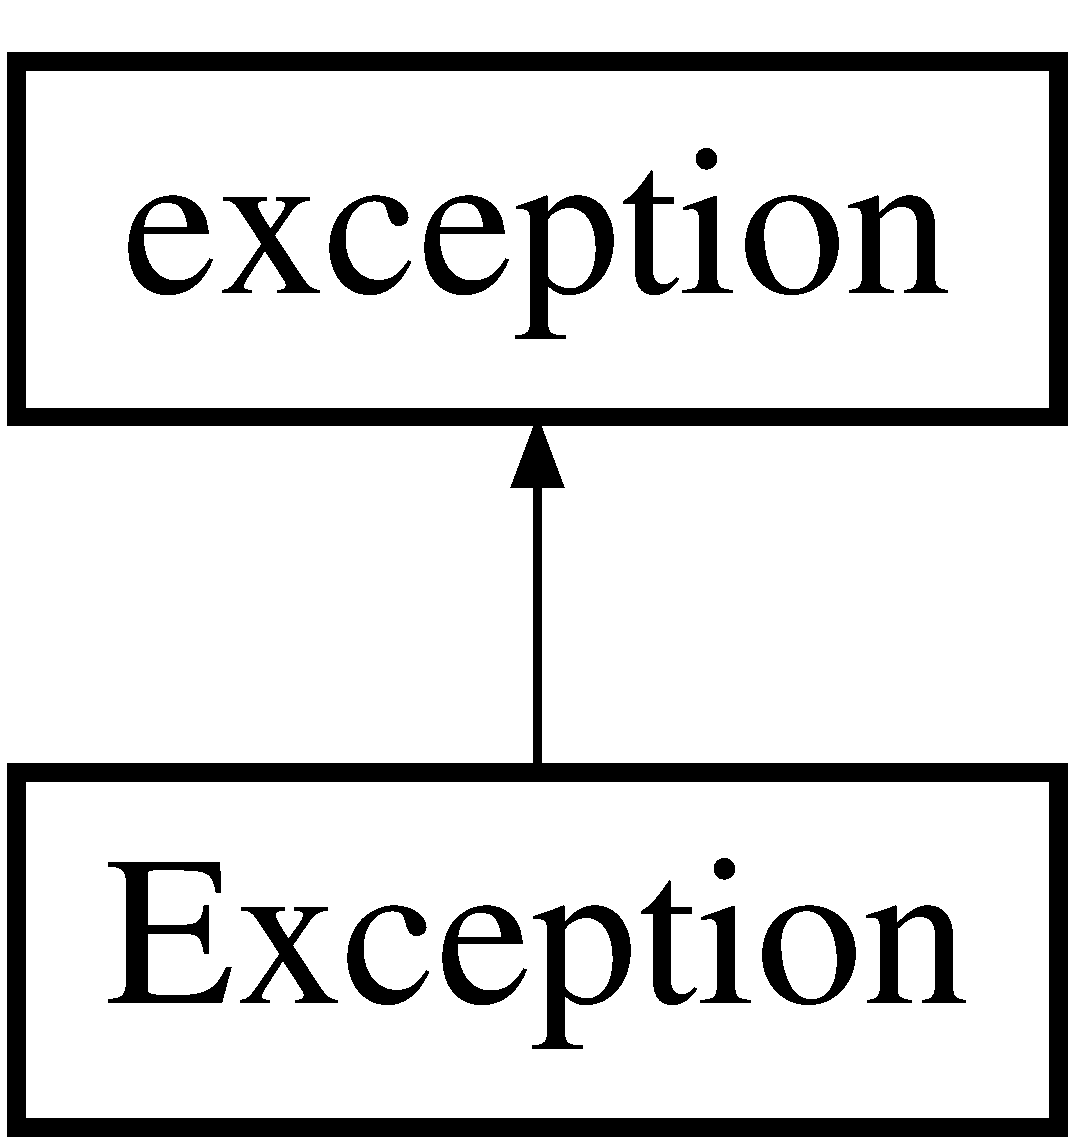
\includegraphics[height=2.000000cm]{class_exception}
\end{center}
\end{figure}
\subsection*{Public Member Functions}
\begin{DoxyCompactItemize}
\item 
\mbox{\Hypertarget{class_exception_a024d3acad826f88c249b8969f90ebb5b}\label{class_exception_a024d3acad826f88c249b8969f90ebb5b}} 
{\bfseries Exception} (const char $\ast$msg)
\item 
\mbox{\Hypertarget{class_exception_a13c431600678afff2c9bd596ec97d2ee}\label{class_exception_a13c431600678afff2c9bd596ec97d2ee}} 
const char $\ast$ {\bfseries what} ()
\end{DoxyCompactItemize}


The documentation for this class was generated from the following files\+:\begin{DoxyCompactItemize}
\item 
inc/Exception.\+hpp\item 
src/Exception.\+cpp\end{DoxyCompactItemize}

\hypertarget{class_logon}{}\section{Logon Class Reference}
\label{class_logon}\index{Logon@{Logon}}
\subsection*{Static Public Member Functions}
\begin{DoxyCompactItemize}
\item 
\mbox{\Hypertarget{class_logon_aebfff5adecbc80681a654ed9d4d5ecf6}\label{class_logon_aebfff5adecbc80681a654ed9d4d5ecf6}} 
static void {\bfseries sign\+\_\+in} ()
\item 
\mbox{\Hypertarget{class_logon_a531b1b7853c47c35a4a89c56250dd650}\label{class_logon_a531b1b7853c47c35a4a89c56250dd650}} 
static void {\bfseries sign\+\_\+up} ()
\item 
\mbox{\Hypertarget{class_logon_a8786b259d84a281e3aa0e617d29a5e8b}\label{class_logon_a8786b259d84a281e3aa0e617d29a5e8b}} 
static bool {\bfseries verify\+\_\+client} (string cpf)
\item 
\mbox{\Hypertarget{class_logon_aa89a2e6fb9631562485c38b5533f0616}\label{class_logon_aa89a2e6fb9631562485c38b5533f0616}} 
static bool {\bfseries validate\+\_\+cpf} (const string \&cpf)
\item 
\mbox{\Hypertarget{class_logon_ad2419d09493bf5da6b6ff7b9e79cc646}\label{class_logon_ad2419d09493bf5da6b6ff7b9e79cc646}} 
static vector$<$ \hyperlink{class_client}{Client} $>$ {\bfseries get\+\_\+client\+\_\+list} ()
\item 
\mbox{\Hypertarget{class_logon_a79e6acb6429d4bc902970a01a6827f4a}\label{class_logon_a79e6acb6429d4bc902970a01a6827f4a}} 
static vector$<$ \hyperlink{class_client}{Client} $>$ {\bfseries read\+\_\+file} (string file\+\_\+name)
\item 
\mbox{\Hypertarget{class_logon_aea874971c4eeaad12528c38e5d72b00e}\label{class_logon_aea874971c4eeaad12528c38e5d72b00e}} 
static void {\bfseries write\+\_\+file} (string file\+\_\+name, \hyperlink{class_client}{Client} client)
\item 
\mbox{\Hypertarget{class_logon_a456f7f498f6395bbe3166b0ebde26d29}\label{class_logon_a456f7f498f6395bbe3166b0ebde26d29}} 
static void {\bfseries over\+Write\+\_\+file} (string file\+\_\+name, vector$<$ \hyperlink{class_client}{Client} $>$ list)
\end{DoxyCompactItemize}


The documentation for this class was generated from the following files\+:\begin{DoxyCompactItemize}
\item 
inc/Logon.\+hpp\item 
src/Logon.\+cpp\end{DoxyCompactItemize}

\hypertarget{class_product}{}\section{Product Class Reference}
\label{class_product}\index{Product@{Product}}
\subsection*{Public Member Functions}
\begin{DoxyCompactItemize}
\item 
\mbox{\Hypertarget{class_product_a9a8cdf5088bfb564bfcede52ab240152}\label{class_product_a9a8cdf5088bfb564bfcede52ab240152}} 
{\bfseries Product} (string product\+\_\+name, string category, double price, int amount)
\item 
\mbox{\Hypertarget{class_product_abf49afaa9cbb5feba6104434c4092fc0}\label{class_product_abf49afaa9cbb5feba6104434c4092fc0}} 
void {\bfseries display\+Product} ()
\item 
\mbox{\Hypertarget{class_product_a23ab3e0728d0d706db6e36c1a14724f7}\label{class_product_a23ab3e0728d0d706db6e36c1a14724f7}} 
string {\bfseries get\+\_\+product\+\_\+name} ()
\item 
\mbox{\Hypertarget{class_product_acf88da4625579cea22785c9a34052aa0}\label{class_product_acf88da4625579cea22785c9a34052aa0}} 
void {\bfseries set\+\_\+product\+\_\+name} (string product\+\_\+name)
\item 
\mbox{\Hypertarget{class_product_ae8c8973a1565b81b0874e724c44116da}\label{class_product_ae8c8973a1565b81b0874e724c44116da}} 
string {\bfseries get\+\_\+category} ()
\item 
\mbox{\Hypertarget{class_product_a7f0b82d1f3ee2c46c69c5c7903e12400}\label{class_product_a7f0b82d1f3ee2c46c69c5c7903e12400}} 
void {\bfseries set\+\_\+category} (string category)
\item 
\mbox{\Hypertarget{class_product_ae83c8f49770a528daa17e5cc27c473e3}\label{class_product_ae83c8f49770a528daa17e5cc27c473e3}} 
double {\bfseries get\+\_\+price} ()
\item 
\mbox{\Hypertarget{class_product_a83f48e73ee9dfa716a864d316ad13b42}\label{class_product_a83f48e73ee9dfa716a864d316ad13b42}} 
void {\bfseries set\+\_\+price} (double price)
\item 
\mbox{\Hypertarget{class_product_ae84c2108928c2b422248b1120a5b2e07}\label{class_product_ae84c2108928c2b422248b1120a5b2e07}} 
int {\bfseries get\+\_\+amount} ()
\item 
\mbox{\Hypertarget{class_product_a8149750b2c12563ebeb7e8ebdaf728ba}\label{class_product_a8149750b2c12563ebeb7e8ebdaf728ba}} 
void {\bfseries set\+\_\+amount} (int amount)
\item 
\mbox{\Hypertarget{class_product_a7dead85ab9565147101d963dd002a137}\label{class_product_a7dead85ab9565147101d963dd002a137}} 
bool {\bfseries operator==} (\hyperlink{class_product}{Product} \&obj)
\end{DoxyCompactItemize}
\subsection*{Friends}
\begin{DoxyCompactItemize}
\item 
\mbox{\Hypertarget{class_product_ad5a69cc0f60cb5ba3b01d430384efa47}\label{class_product_ad5a69cc0f60cb5ba3b01d430384efa47}} 
ostream \& {\bfseries operator$<$$<$} (ostream \&out, const \hyperlink{class_product}{Product} \&obj)
\item 
\mbox{\Hypertarget{class_product_a0db1f7f5144f31ac438bf5ffdb70fc87}\label{class_product_a0db1f7f5144f31ac438bf5ffdb70fc87}} 
istream \& {\bfseries operator$>$$>$} (istream \&in, \hyperlink{class_product}{Product} \&obj)
\end{DoxyCompactItemize}


The documentation for this class was generated from the following files\+:\begin{DoxyCompactItemize}
\item 
inc/Product.\+hpp\item 
src/Product.\+cpp\end{DoxyCompactItemize}

\hypertarget{class_stock}{}\section{Stock Class Reference}
\label{class_stock}\index{Stock@{Stock}}
\subsection*{Static Public Member Functions}
\begin{DoxyCompactItemize}
\item 
\mbox{\Hypertarget{class_stock_a0d315ad78d90d7b44b03ee205901167c}\label{class_stock_a0d315ad78d90d7b44b03ee205901167c}} 
static void {\bfseries add\+\_\+product} ()
\item 
\mbox{\Hypertarget{class_stock_a63c7f5ff4735d7c432513a184cc1f8ae}\label{class_stock_a63c7f5ff4735d7c432513a184cc1f8ae}} 
static void {\bfseries restock} ()
\item 
\mbox{\Hypertarget{class_stock_a723436b7d02d654b44240a8a9b299b53}\label{class_stock_a723436b7d02d654b44240a8a9b299b53}} 
static bool {\bfseries verify\+\_\+stock} (string product\+\_\+name)
\item 
\mbox{\Hypertarget{class_stock_a656392425435a9c6d4b2c11701bd874a}\label{class_stock_a656392425435a9c6d4b2c11701bd874a}} 
static bool {\bfseries verify\+\_\+amount} (\hyperlink{class_product}{Product} product, int amount)
\item 
\mbox{\Hypertarget{class_stock_a697aae3215e7c4f3f2de2ad54e8ec679}\label{class_stock_a697aae3215e7c4f3f2de2ad54e8ec679}} 
static vector$<$ \hyperlink{class_product}{Product} $>$ {\bfseries get\+\_\+stock} ()
\item 
\mbox{\Hypertarget{class_stock_aebee78521677e6ec8d3d3dafe07b2246}\label{class_stock_aebee78521677e6ec8d3d3dafe07b2246}} 
static vector$<$ \hyperlink{class_product}{Product} $>$ {\bfseries read\+\_\+file} (string file\+\_\+name)
\item 
\mbox{\Hypertarget{class_stock_adcde805388eaefb2da64afae6960c8d8}\label{class_stock_adcde805388eaefb2da64afae6960c8d8}} 
static void {\bfseries write\+\_\+file} (string file\+\_\+name, \hyperlink{class_product}{Product} product)
\item 
\mbox{\Hypertarget{class_stock_ab9eca0846f29c41181a63aff568c61be}\label{class_stock_ab9eca0846f29c41181a63aff568c61be}} 
static void {\bfseries over\+\_\+write} (string file\+\_\+name, vector$<$ \hyperlink{class_product}{Product} $>$ list)
\end{DoxyCompactItemize}


The documentation for this class was generated from the following files\+:\begin{DoxyCompactItemize}
\item 
inc/Stock.\+hpp\item 
src/Stock.\+cpp\end{DoxyCompactItemize}

\hypertarget{class_store}{}\section{Store Class Reference}
\label{class_store}\index{Store@{Store}}
\subsection*{Static Public Member Functions}
\begin{DoxyCompactItemize}
\item 
\mbox{\Hypertarget{class_store_af47a60a210ac3c173f4b1d341e156d6b}\label{class_store_af47a60a210ac3c173f4b1d341e156d6b}} 
static void {\bfseries start\+\_\+session} ()
\item 
\mbox{\Hypertarget{class_store_a25bb5f118c857559dac732a8060492c3}\label{class_store_a25bb5f118c857559dac732a8060492c3}} 
static void {\bfseries main\+\_\+menu} ()
\item 
\mbox{\Hypertarget{class_store_a315768e57e06ea5de3e0ab8ccc224356}\label{class_store_a315768e57e06ea5de3e0ab8ccc224356}} 
static void {\bfseries shop\+\_\+mode} ()
\item 
\mbox{\Hypertarget{class_store_a6d3e577633bb7636bbf8bb46163eed6b}\label{class_store_a6d3e577633bb7636bbf8bb46163eed6b}} 
static void {\bfseries stock\+\_\+mode} ()
\item 
\mbox{\Hypertarget{class_store_a44626a175e2bf648fc11749a156bb68f}\label{class_store_a44626a175e2bf648fc11749a156bb68f}} 
static void {\bfseries recommendation\+\_\+mode} ()
\item 
\mbox{\Hypertarget{class_store_aae0571b011a7a886d5ee27477796911b}\label{class_store_aae0571b011a7a886d5ee27477796911b}} 
static void {\bfseries input\+\_\+option} (const int \&n\+\_\+options, const string \&e\+\_\+message)
\end{DoxyCompactItemize}


The documentation for this class was generated from the following files\+:\begin{DoxyCompactItemize}
\item 
inc/Store.\+hpp\item 
src/Store.\+cpp\end{DoxyCompactItemize}

%--- End generated contents ---

% Index
\backmatter
\newpage
\phantomsection
\clearemptydoublepage
\addcontentsline{toc}{chapter}{Index}
\printindex

\end{document}
